%----------------------------------------------------------------
%
%  File    :  thesis-style.tex
%
%  Author  :  Keith Andrews, IICM, TU Graz, Austria
%
%  Created :  27 May 93
%
%  Changed :  19 Feb 2004
%
% styling and technical implementation adopted 2011 by Karl Voit
%----------------------------------------------------------------
\newpage
\section{Lineare Bauelemente}


\subsection{Kondensator}
\definition{Kapazität}
\beginip
	Die elektrische Kapazität C beschreibt die Fähigkeit eines Bauelementes, Ladung $Q$ bei einer gewissen Spannung $U$ zu speichern.
	\formulaBegin
	$C =\displaystyle \frac{Q}{U} \underbrace{=}_{Plattenkondensator} \varepsilon \frac{A}{d}$
	\formulaEnd
	Die in einer Kapazität gespeicherte Energie berechnet sich als
	\formulaBegin
	$W =\displaystyle \frac{1}{2}C \cdot U^2$
	\formulaEnd
\iend


\definition{Serienschaltung von Kapazitäten}

\beginip
Werden mehrere Kapazitäten seriell miteinander verbunden, so addieren sich die Kehrwerte der Kapazität \\
\formulaBegin
$\displaystyle \frac{1}{C_{ges}} = \sum_{i=0}^n \frac{1}{C_i} \Bigg\rvert$
$\displaystyle C_{ges} = \frac{C_1 \cdot C_2}{C_1 + C_2} = (C_1 || C_2)$
\formulaEnd
\iend


\textbf{Begründung} \\
 	Die Definition der Kapazität ist genau gegensätzlich zu der des Widerstandes ($ R \propto \frac{l}{A}$ , $ C \propto \cdot \frac{A}{d} $)\\
	 Werden Kondensatoren in Serie geschaltet, so vergrößert sich der effektive Abstand der Platten, weshalb wir die Kehrwerte addieren müssen. \\



	\definition{Parallelschaltung von Kapazitäten}

	\beginip
	Werden mehrere Kapazitäten parallel miteinander verbunden, so addieren sich die Kapazitäten \\
	\formulaBegin
	$\displaystyle C_{ges} = \sum_{i=0}^n C_i x$
	\formulaEnd
	\iend

\newpage
	\definition{Ladungserhaltung in der Serienschaltung}
	\beginip
		Werden Kapazitäten in Serie geschaltet, besitzen alle dieselbe Ladung Q.
		\begin{center}
			\fix
				\ibox{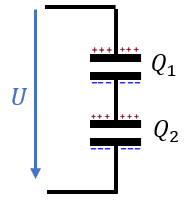
\includegraphics[scale=0.5]{img/kond1.png}} $\displaystyle \doubleunderline{Q_1 = Q_2 = Q}$
		\end{center}
	\iend

	\textbf{Begründung} \\
		Damit sich auf dem ersten Kondensator die Ladung $Q_1$ ansammeln kann, muss diese Ladung unterhalb des Kondensators angesammelt werden. Angenommen, beide Kondensatoren waren zu Beginn ungeladen,
		so muss die Ladung, welche sich auf der unteren Platte des ersten Kondensators befindet, dieselbe Ladungsmenge auf der oberen Platte des unteren Kondensators hervorrufen. \\

		\definition{Maschenregel bei Parallelschaltung}
		\beginip
			Die Maschenregel für Spannung gilt auch bei Kondensatoren
			\begin{center}
				\fix
					\ibox{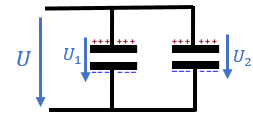
\includegraphics[scale=0.5]{img/kond2.png}}
					$\displaystyle \doubleunderline{U_1 = U_2 = U} $  und  $\displaystyle C_1 = \frac{Q_1}{U_1} \rightarrow \doubleunderline{Q_1 = C_1 \cdot U}$
			\end{center}
		\iend

		\definition{Grundlegende Gleichung am Kondensator}

		\beginip
		Der Zusammenhang zwischen Strom und Spannung am Kondensator ist wie folgt gegeben
		\formulaBegin
		$\displaystyle u_c(t) = \frac{1}{C} \int_0^t i_c(t) dt$ \\

		$\displaystyle i_c(t) = c \cdot \frac{d}{d t} (u_c)$ \\
		\formulaEnd
		\iend
		\textbf{Begründung} \\
			Mit dem Wissen, dass Strom definiert ist als die Ladung pro Zeit $ \displaystyle \frac{dQ}{dt} = I$ folgt folgendes: \\
			\begin{center}
				\fix
			$\displaystyle \frac{\partial}{\partial t} (C \cdot U) = \frac{\partial}{\partial t} (Q) $ \\
			$ \displaystyle C  \cdot \frac{dU}{dt} = I \rightarrow U(t) = \frac{1}{C} \cdot \int_0^t I \cdot dt$
		\end{center}


\newpage
	\textbf{Übersicht} \\
	\\
	\begin{tabular}{|c|c|c|c|c|}
	\hline
		\textbf{Energie} & 	\textbf{Strom und Spannung} & 	\textbf{ DC-Verhalten} & 	\textbf{ High-AC Verhalten*}& 	\textbf{ Admitanz*} \\
		\hline 	\hline
		 & & & & \\
	    $ \displaystyle C =  \frac{Q}{U} $ & $\displaystyle u_c(t) = \frac{1}{C} \int_0^t i_c(t) dt $ & Leerlauf & Kurzschluss & $ \displaystyle \frac{1}{j\omega C}$  \\
		  $\displaystyle W =  \frac{1}{2} C U^2 $ & $\displaystyle i_c(t) = c \cdot \frac{d}{d t} (u_c) $ & 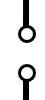
\includegraphics[scale=0.4]{img/leerlauf} &  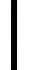
\includegraphics[scale=0.5]{img/kurzschluss} &   \\
			 & & & & \\
			\hline
	\end{tabular}




\newpage






\subsection{Magnetostatik}

	Analog zum elektrischen Feld definieren wir ein magnetisches Feld, dessen Feldlinien Kräfte auf eine bewegte Ladung auswirken. \\
	Auslöser für das magnetische Feld sind \textbf{bewegte Ladungen} welche gemäss der rechten Hand Regel ein Magnetfeld hervorrufen, das diese einschliesst. \\
	Im Falle von Stabmagneten oder 	Ähnlichem ist es der Spin der Elektronen, welcher das stationäre Magnetfeld auslöst*\\

	\definition{Rechte Hand Regel}
	\beginip
	Das Magnetfeld $B$ um einen stromdurchflossenen Leiter baut sich stets gegen den Uhrzeigersinn auf und ist \textbf{immer} geschlossen. \\
	\begin{center}
			\ibox{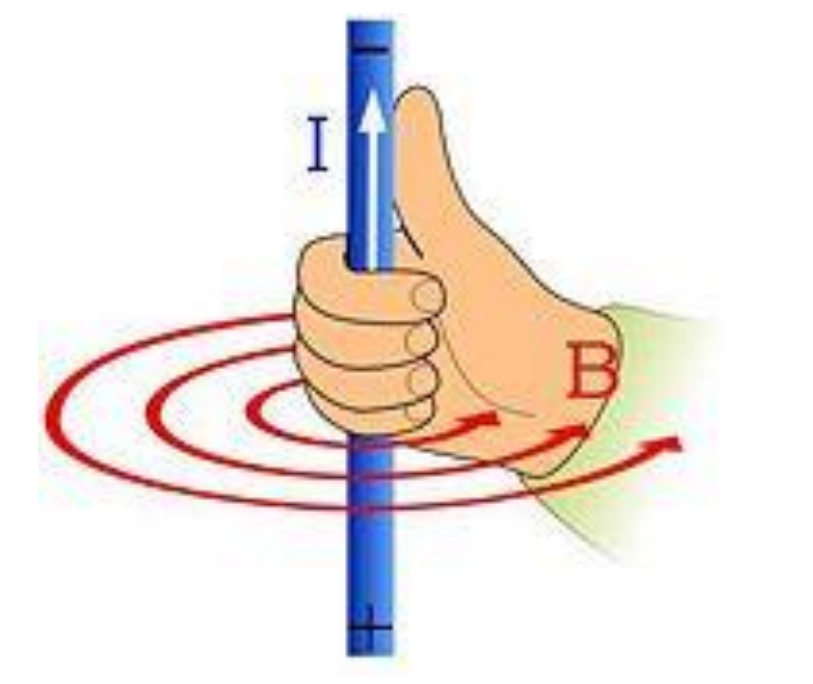
\includegraphics[scale=0.2]{img/rechte-hand-regel.png}}
	\end{center}
	\iend

	\definition{Lorentzkraft}
	\beginip
	Bewegte Ladungen in einem Magnetfeld verspüren eine Kraft, welche proportional zur Stärke des B-Feldes und der Geschwindigkeit ist. \\
	Die Kraft steht senkrecht zu den Feld- und Geschwindigkeits-Vektoren.

	\formulaBegin
	$\vec{F_L} = q \cdot \vec{v} \times \vec{B} = I(\vec{l} \times \vec{B})$
	\formulaEnd

	\begin{center}
			\ibox{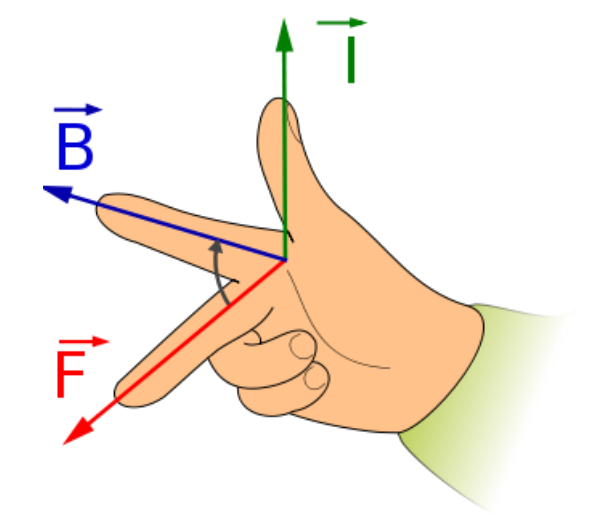
\includegraphics[scale=0.3]{img/lorentzkraft.png}}
	\end{center}
	\iend

\newpage
	\definition{H-Feld}
	\beginip
	Legen wir ein magnetisches Feld an eine Materie an, so richten sich die eingeschlossenen Teile entgegen dem angelegten Feld aus und \texttt{"} schwächen \texttt{"} dieses. \\
	Das \texttt{"} abgeschwächte \texttt{"} Feld bezeichnen wir als H-Feld und entspricht dem Feld, welches real auf Ladungen wirkt. \\
	 Der \texttt{"}Abschwächungsfaktor\texttt{"} $\mu = \mu_0 \cdot \mu_r$ wird als Permeabilität bezeichnet. \\
	 Das H-Feld verändert sich bei Materialübergängen, das \textbf{B-Feld} bleibt \textbf{konstant}.

	\formulaBegin
	$\displaystyle \vec{H} = \frac{\vec{B}}{\mu}$
	\formulaEnd

	\begin{center}
			\ibox{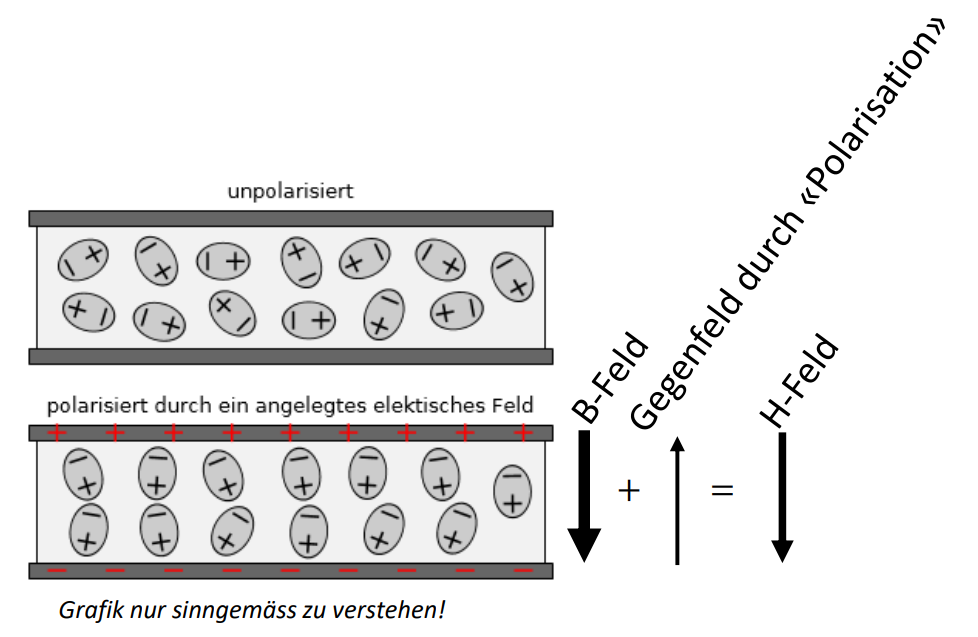
\includegraphics[scale=0.4]{img/h-feld.png}}
	\end{center}
	\iend

	\definition{Durchflutungssatz}
	\beginip
	Der Durchflutungssatz besagt, dass das Kurvenintegral des H-Feldes über eine beliebige \textbf{geschlossene} Kurve gerade dem Wert des durch diese Fläche fließendes Stromes entspricht. \\
	Diesen Wert definieren wir als magnetische Spannung $\Theta$ \\
	\formulaBegin
	$\displaystyle \Theta = \oint_{\partial A} \vec{H} \cdot d\vec{s} = \iint_{A} \vec{j} \cdot d\vec{A} $
	\formulaEnd
	\iend

	\important{Beispiel}{\#4}
	\beginip
	\textbf{Aufgabe} \\
	Berechnen Sie die magnetische Spannung $\Theta$ und das H-Feld Feld $\vec{H}$ um einen unendlich langen, mit Strom I durchflossenen Leiter. Der Radius des Leiters sei $\rho$. \\
	\iend

	\beginip
	\textbf{Lösung} \\

	Wir wählen als Kurve einen Kreis mit Radius R um unseren Leiter. \\
	Da wir von einem perfekten Leiter ausgehen, treffen wir die Annahme, dass das Magnetfeld achsensymmetrisch und somit konstant entlang des Kreises ist. \\
	\\
	Wir erhalten: für R $ > \rho$: \\
	$\displaystyle  \doubleunderline{\Theta} =  \oint_{2\pi R} \vec{H} \cdot d\vec{S} = \doubleunderline{I} $ \\
	$ \displaystyle \rightarrow |H| \cdot 2 \pi R = I \rightarrow \doubleunderline{\vec{H}(R) = \frac{I}{2 \pi R} \cdot \vec{e_{\varphi}}} $\\

	Für R $ < \rho $ : \\
	$\displaystyle  \doubleunderline{\Theta(R)} =  \oint_{2\pi R} \vec{H} \cdot d\vec{S} =\int_{0}^{R} \int_{0}^{2\pi} \frac{I}{\pi{\rho}^2} \cdot r \cdot d\varphi  \cdot dr  = \frac{2 \cdot I}{\rho^2} \cdot \frac{1}{2} R^2 =  \doubleunderline{\frac{R^2\cdot I}{\rho^2}} 		  $ \\
	$ \displaystyle \rightarrow |H| \cdot 2 \pi R = \frac{I \cdot R^2}{\rho^2} \rightarrow \doubleunderline{\vec{H}(R) = \frac{I}{2\pi \rho^2} \cdot R \cdot \vec{e_{\varphi}}} $

	\textbf{Skizze}
	\begin{center}
		\ibox{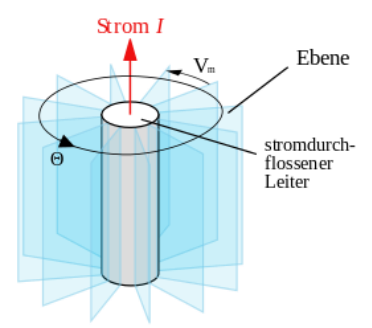
\includegraphics[scale=0.7]{img/ex4-1.png}}
	\end{center}
	\iend

	\important{Magnetische Spannung innerhalb einer Spule}{}

	\beginip
	Analog zu den Berechnungen beim Leiter kann man die magnetische Spannung innerhalb einer Spule berechnen. Unter der Annahme, dass das magnetische Feld ausserhalb des Spule vernachlässigbar ist
	und die Spule N Windungen hat, erhalten wir für den Fluss durch das Innere einer Spule:

	\formulaBegin
	$\displaystyle \Theta_{Spule} = \oint_{\partial A} \vec{H} \cdot d\vec{s} = \iint_{A} \vec{j} \cdot d\vec{A} = N \cdot I \simeq \int_0^b \vec{H} \cdot d\vec{s}$
	\formulaEnd
	\begin{center}
		\ibox{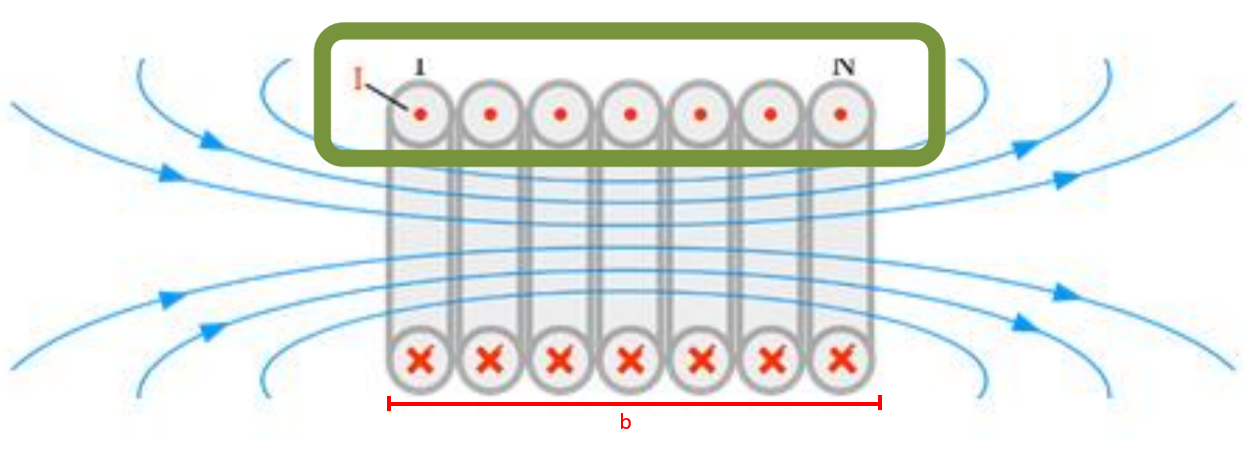
\includegraphics[scale=0.3]{img/spule_fluss.png}}
	\end{center}
	\iend

	Im folgenden gehen wir davon aus, dass die magnetische Spannung ungefähr $ \Theta = \int_0^l \vec{H} d\vec{s}$ entspricht.\\
	\definition{magnetischer Fluss}
	\beginip
		Als magnetischen Fluss $\Phi$ bezeichnen wir die \texttt{"}Menge B-Feld\texttt{"}, welche durch eine gegebene Fläche fliesst. \\
		\formulaBegin
		$\displaystyle \Phi := \iint_A \vec{B} \cdot \vec{n} \cdot da$
		\formulaEnd
	\iend


	\definition{magnetischer Widerstand}
		\beginip
			Als magnetischer Widerstand $R_m$ bezeichnen wir das Verhältnis zwischen magnetischer Spannung und magnetischem Fluss \\
			Er sagt etwas darüber aus, wie gross der magnetische Fluss bei einer gegebenen magnetischen Spannung ist.
			\formulaBegin
			$\displaystyle R_m = \frac{\Theta}{\Phi} \underbrace{=}_{magn. Leiter} \frac{l}{\mu \cdot A}$
			\formulaEnd
		\iend

		\textbf{Begründung} \\
		Wir gehen davon aus, dass die magnetische Spannung über einem Leiter mit Länge l anliegt, dessen Querschnittfläche A ist. \\
		\begin{center}
			$\displaystyle \frac{\Theta}{\Phi} = \frac{\int_0^l \vec{H} \cdot d\vec{s}}{\iint_a \vec{B} d \vec{A}} = \frac{l \cdot H}{\mu \cdot A \cdot H} = \frac{l}{\mu \cdot A} $

		\end{center}


\newpage

\subsubsection{Das Reluktanzmodell}
		\textbf{magnetische Grössen im Vergleich zu eletrischen} \\

		\def\arraystretch{2}%  1 is the default, change whatever you need
		\begin{tabular}{c|c|c||c|c}
			& Elektrisch & Einheit & Magnetisch & Einheit \\
			\hline
			\hline
			Leitfähigkeit & $ \kappa $ & $\texttt{[}   \frac{1}{\Omega \cdot m}    \texttt{]}$ & $\mu (= \mu_0 \cdot \mu_r)$ & $\texttt{[}  \frac{H}{m}\texttt{]}$ \\
			Widerstand & $ R = \frac{l}{\kappa A} $ & $\texttt{[}   \Omega   \texttt{]}$ & $R_m = \frac{l}{\mu A}$ & $\texttt{[} \frac{1}{H}\texttt{]}$ \\
			Leitwert & $ G = \frac{1}{R} $ & $\texttt{[}  S \texttt{]}$ & $\Lambda_m = \frac{1}{R_m}$ & $\texttt{[}  H  \texttt{]}$ \\
			\hline


			Spannung & $\displaystyle U_{AB} = \int_A^B \vec{E} \cdot d\vec{s}$ & $\texttt{[}V\texttt{]}$ & $\displaystyle \Theta_{AB}= \int_A^B \vec{H} \cdot d\vec{s}$ &  $\texttt{[}A\texttt{]}$ \\
			Strom / Fluss & $\displaystyle I = \iint_A \vec{j}\cdot d\vec{A} = \kappa \iint_A \vec{E} \cdot d\vec{A}$ & $\texttt{[}A\texttt{]}$  & $ \iint_A \vec{B} \cdot d \vec{A} = \mu \iint_A \vec{H} \cdot d\vec{A}$ &  $\texttt{[}Wb\texttt{]}$ \\
			\hline
			Ohmsches Gesetz & $U = R \cdot I $ &  & $\Theta = R_m \cdot \Phi $ &  \\
			Maschenregel & $ U_0 = \sum_{Masche} U_m $ &  & $ \Theta(= NI) = \sum_{Masche} \Theta_m $ & \\
			Knotenregel & $ \sum_{Knoten} I_k = 0 $ &  & $ \sum_{Knoten} \Phi_k = 0 $ &  \\

		\end{tabular}

		\definition{Reluktanzmodell}
		\beginip
		Das Reluktanzmodell besagt, dass man ein magnetisches Ersatzschaltbild mit denselben Rechenregeln wie bei einem elektrischen Netzwerk berechnen kann. \\
		\textbf{Vorgehen} \\
		\begin{itemize}
			\item Spulen werden mit Spannungsquellen ersetzt $V_m = N\cdot I$
			\item Magnetkerne/Luftspälte etc. werden mithilfe der Länge und Querschnittsfläche als Widerstände modelliert. $R_m = \mu \frac{l}{A}$
			\item Für magnetische Widerstände gelten die gleichen Regeln wie bei elektrischen (Seriellschaltung / Paralellschaltung).
		\end{itemize}

		\iend
\newpage
		\important{Beispiel}{\#5}
		\beginip
 		\textbf{Aufgabe Hubmagnet} \\
		Der mittlere Schenkel 2 eines E-Kernes aus Dynamoblech trägt eine Wicklung mit N Windungen. Über
		die drei Luftspalten mit gleicher Länge $\delta$ wird ein Anker aus Grauguss mit der Kraft FA angezogen
		E-Kern und Anker besitzen die gleiche Dicke d. \\
		\begin{center}
		\ibox{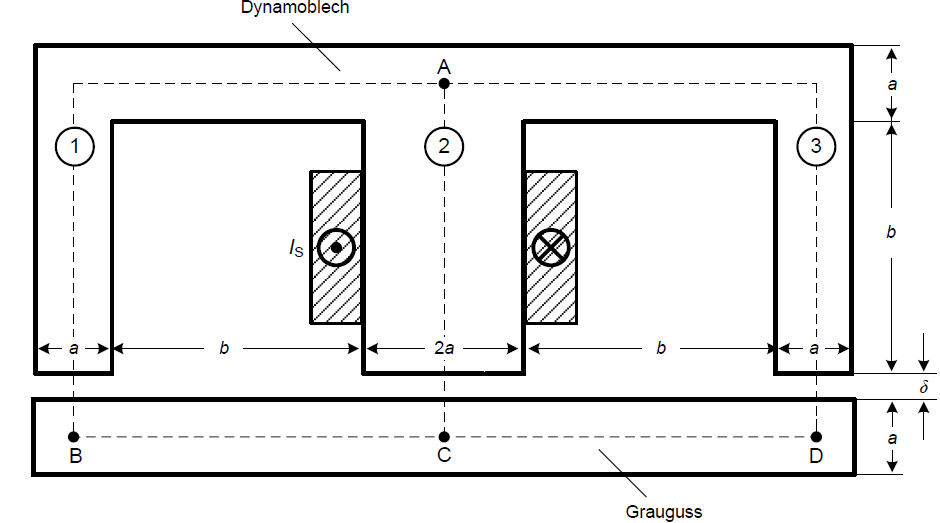
\includegraphics[scale=0.4]{img/ex5-1.png}}
		\end{center}
		Gegeben sind folgende Parameter: \\

		\begin{center}
	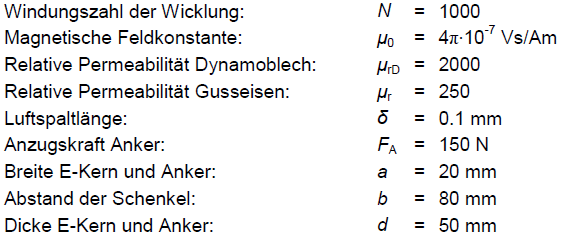
\includegraphics[scale=0.6]{img/ex5-3.png}
		\end{center}
		Berechnen sie die magnetische Spannung auf dem Weg ACD.
		\iend

\newpage
		\important{Lösung}{}
				\beginip
		Zuerst zeichnen wir ein Reluktanzmodell des Magneten. \\
		Wobei $R_L$ die Luftspälte, ${R_D}_i$ die Beine des Magneten und ${R_G}_i$ sowie $R_{BC}$ und $R_{CD}$ das Gusseinsenstück modellieren.
	\begin{center}
			\ibox{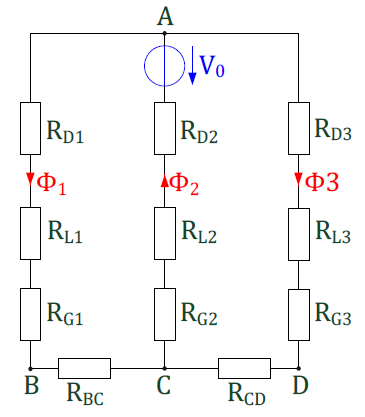
\includegraphics[scale=0.5]{img/ex5-2.png}}
			\end{center}


		Für die Spannungsquelle erhalten wir:
			\begin{center}

				 $V_0 = N \cdot I_s = 1000 \cdot 211.3mA = 211.3A$ \\
			\end{center}
		Für die Widerstände:
			\begin{center}
	 	$R_{D1} = R_{D3} = \frac{2b + 2a}{\mu_0 \mu_{rD} a d} = 79.6 \cdot 10^3H^{-1}$ \\
	 	$R_{D2} = \frac{b + \frac{a}{2} }{2 \mu_0 \mu_{rD} a d} = 17.9 \cdot 10^3H^{-1}$ \\

	 	$R_{L1} = R_{L3} = \frac{\delta}{\mu_0 a d} = 79.6 \cdot 10^3H^{-1}$ \\
		$R_{L2} =  \frac{\delta}{2\mu_0 a d} = 39.8 \cdot 10^3 H^{-1}$\\
		$R_{G1} = R_{G3} = \frac{\frac{a}{2}}{\mu_0\mu_{rG}ad} = 31.8 \cdot 10^3H^{-1}$ \\
		$R_{G2} =\frac{\frac{a}{2}}{2\mu_0\mu_{rG}ad} = 15.9 \cdot 10^3H^{-1}$ \\
		$R_{BC} = R_{CD} = \frac{b + \frac{3}{2}a}{2\mu_0\mu_{rG}ad} = 350.1\cdot 10^3H^{-1}$ \\
				\end{center}
		Weiter können wir die einzelnen Widerstände seriell zusammenfassen:
			\begin{center}
		$R_1 = R_{D1} + R_{L1} + R_{G1} = 191 \cdot 10^3 H^{-1}$ \\
		$R_2 = R_{D2} + R_{L2} + R_{G2} = 73.7 \cdot 10^3 H^{-1}$ \\
		$R_3 = R_{D3} + R_{L3} + R_{G3} = 191 \cdot 10^3 H^{-1}$ \\
		$R_E = R_{BC} = R_ {CD} = 350.1 \cdot 10^3 H^{-1} $ \\
					\end{center}

		Die Spannung $U_{AC}$ lässt sich als Spannungsteiler berechnen:

			\begin{center}
		$\displaystyle U_{AC} = U_0 \cdot \frac{((R_1 + R_E) || (R_3 + R_E)) } { ((R_1 + R_E) || (R_3 + R_E)) + R_2} = 166A$ \\
				\end{center}
		Und somit die Spannung $ U_{AD}$:
		\begin{center}
			$\displaystyle \doubleunderline{U_{AD}} = 166A \cdot \frac{R_1}{R_1 + R_E} = \doubleunderline{58.6A}$
		\end{center}
		\iend

\newpage

\subsection{Spule und Induktivität}

\definition{Induktivität}
\beginip
	Die Induktivität L beschreibt, wieviel magnetischer Fluss $\Phi$ sich bei einem Strom I im Inneren eines Bauteiles aufbaut.
	\formulaBegin
	$ L := \frac{N\cdot \Phi}{I} = \frac{N^2}{R_m} $
	\formulaEnd
	Die in einer Induktivität gespeicherte Energie berechnet sich zu
	\formulaBegin
	$W =\displaystyle \frac{1}{2}L \cdot I^2$
	\formulaEnd
\iend



	\definition{Serien und Parallelschaltung}
	 \beginip
	 	Induktivitäten verhalten sich analog zu Widerständen: \\
		\textbf{Serienschaltung}
		\formulaBegin
		$ L_{serie} = \sum_{i=0}^n L_i $
		\formulaEnd

		\textbf{Parallelschaltung}
		\formulaBegin
		$\displaystyle \frac{1}{L_{ges}} = \sum_{i=0}^n \frac{1}{L_i} \Bigg\rvert L_{p_2} = (L_1 || L_2 )$
		\formulaEnd
	 \iend


	\textbf{Übersicht} \\
	\\
	\begin{tabular}{|c|c|c|c|c|}
	\hline
		\textbf{Energie} & 	\textbf{Strom und Spannung} & 	\textbf{ DC-Verhalten} & 	\textbf{ High-AC Verhalten*}& 	\textbf{ Admitanz*} \\
		\hline 	\hline
		 & & & & \\
	    $ \displaystyle L =  \frac{N \Phi}{I} $ & $\displaystyle i_L(t) = \frac{1}{L} \int_0^t u_c(t) dt $ & Leerlauf & Kurzschluss & $ \displaystyle j\omega L$  \\
		  $\displaystyle W =  \frac{1}{2} L I^2 $ & $\displaystyle u_L(t) = L \cdot \frac{d}{d t} (i_c) $ & 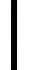
\includegraphics[scale=0.5]{img/kurzschluss} &   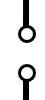
\includegraphics[scale=0.4]{img/leerlauf}  &   \\
			 & & & & \\
			\hline
	\end{tabular}

%
% \section{Transformatoren}
% \definition{Induktionsgesetz}
% \beginip
% Wird eine Leiterschleife oder Spule von einem \textbf{sich änderndem} Magnetischen Fluss durchflossen, so baut sich eine Spannung auf, die proportional zur Änderung des Flusses ist.
%
% \begin{center}
% 	\ibox{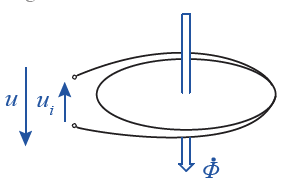
\includegraphics[scale=0.8]{img/induktion_2.png}}
% \end{center}
%
% \formulaBegin
% $\displaystyle u = N \frac{d \Phi}{dt} $
% \formulaEnd
%
% \iend
%
% \definition{Magnetische Koppelung}
%
% 	\beginip
% 		Bringen wir eine Spule oder Leiterschleife in die Nähe einer anderen Spule / Leiterschleife, so wird diese von einem Teil des Flusses der Primärspule ($= \Phi_{21}$) durchflossen. \\
% 		Die Änderung dieses Flusses führt zu einer Änderung des Stromes in der Sekundärspule.
% 			\begin{center}
% 				\ibox{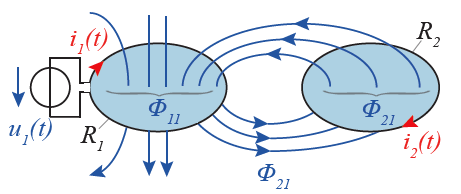
\includegraphics[scale=0.6]{img/koppelung.png}}
% 			\end{center}
% 		\formulaBegin
% 		$\frac{d\Phi_2}{dt} = M_{21} \cdot \frac{di_1}{dt}$
% 		\formulaEnd
%
%
% \iend
%

\newpage
\section{Transiente Vorgänge}
\fix \fix
Transiente Vorgänge sind Ein- oder Ausschaltvorgänge von Schaltungen.
\fix
\subsection{Kondenstor}
\fix
Wir betrachten nun Netzwerke mit einer Quelle, welche einen Innenwiderstand und einen Kondensator enthalten. \\
Das Netzwerk besitzt einen Schalter, womit die Quelle an das Netzwerk angeschlossen oder davon entfernt werden kann. \\
Sollt das Netzwerk aus mehreren Quellen und Widerständen bestehen, so kann mittels Thévenin/Norton Umformung eine einfachere Form erreicht werden.
\definition{Transiente am Kondensator}

\beginip
	Es sei ein Netzwerk der folgenden Form gegeben:
	\begin{center}
		\ibox{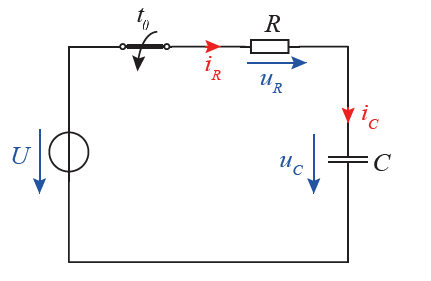
\includegraphics[scale=0.8]{img/transient-kond.png}}
	\end{center}
	Der Schalter werde zum Zeitpunkt $t = t_0$ geschlossen. \\
	Die Spannung am Kondensator beträgt: \\
	\formulaBegin
	$\displaystyle U_C(t) = U_C(\infty) - [u_C(\infty) - u_C(t_0)] \cdot e^{(-\frac{t -t_0}{RC})}$
	\formulaEnd
	Wobei $u_C(\infty)$ die Spannung über dem Kondensator nach dem Einschwingen bezeichnet $(= U)$ und $u_C(t_0)$ die Kondensatorspannung vor dem Schliessen des Schalters.
\iend

\textbf{Begründung} \\
Wir stellen eine Maschengleichung auf: \\
$\displaystyle U = u_R + u_c = i_C \cdot R + u_C = C \cdot R \frac{d}{dt}(u_c) + u_c$ \\
Wir berechnen die hmogene Lösung:  \\
$ \frac{d}{dt}(u_c) + \frac{1}{RC} u_c = 0$ \\
$ u_{c,hom} = A\cdot e^{-\frac{t}{RC}}$ \\
Danach die partikuläre Lösung mit Ansatz $u_c = A + Bt$: \\
$ RC \frac{d}{dt}(u_c) + u_c = U \rightarrow RC \cdot B  + ( A + Bt) = U $ \\
$ \rightarrow u_c(t) = U$ \\
Als Endlösung erhalten wir: \\
$\displaystyle u_c(t) = U + A \cdot  e^{(-\frac{t}{RC})}$

\subsection{Induktivität}
Wir betrachten nun Netzwerke mit einer Quelle, welche einen Innenwiderstand und eine Induktivität enthalten. \\
Das Netzwerk besitzt einen Schalter, womit die Quelle an das Netzwerk angeschlossen oder davon entfernt werden kann. \\
Sollt das Netzwerk aus mehreren Quellen und Widerständen bestehen, so kann mittels Thévenin/Norton Umformung eine einfachere Form erreicht werden.
\definition{Transiente an der Induktivität}

\beginip
	Sei ein Netzwerk der folgenden Form gegeben:
	\begin{center}
		\ibox{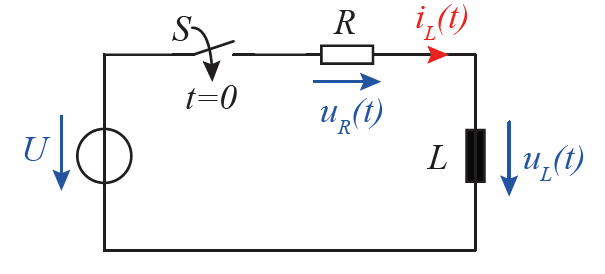
\includegraphics[scale=0.8]{img/transient-indukt.png}}
	\end{center}
	Der Schalter werde zum Zeitpunkt $t = t_0$ geschlossen. \\
	Der Strom durch die Induktivität berechnet sich wie folgt:\\
	\formulaBegin
	$\displaystyle i_L(t \rightarrow \infty) - [i_L(t \rightarrow \infty) - i_L(t \rightarrow t_0)]e^{-R \frac{t -t_0}{L}}$
	\formulaEnd
	Wobei $i_L(t \rightarrow \infty)$ den Strom durch die Spule nach dem Einschwingen bezeichnet $(= \frac{U}{R})$ und $i_L(t \rightarrow t_0)$ den Strom durch die Spule vor dem Schliessen des Schalters.
\iend

\newpage

\section{Komplexe Wechselstromrechnung}


\subsection{Komplexe Zahlen}

Nachfolgend werden alle komplexen Variablen durch einen Unterstrich symbolisiert $\underline{Z}$ \\
\definition{Polarform}

\beginip

Die Polarform beschreibt eine komplexe Zahl mithilfe der Länge und dem Winkel eines Zeigers.
Folgende Zusammenhänge sind gegeben:
\formulaBegin
$\displaystyle \underline{z} = a + b j \underbrace{=}_{Polarform} |\underline{z}| \cdot e^{j \cdot arg(\underline{z})} = r\cdot e^{j\cdot \varphi }$
\formulaEnd
\begin{center}
	\ibox{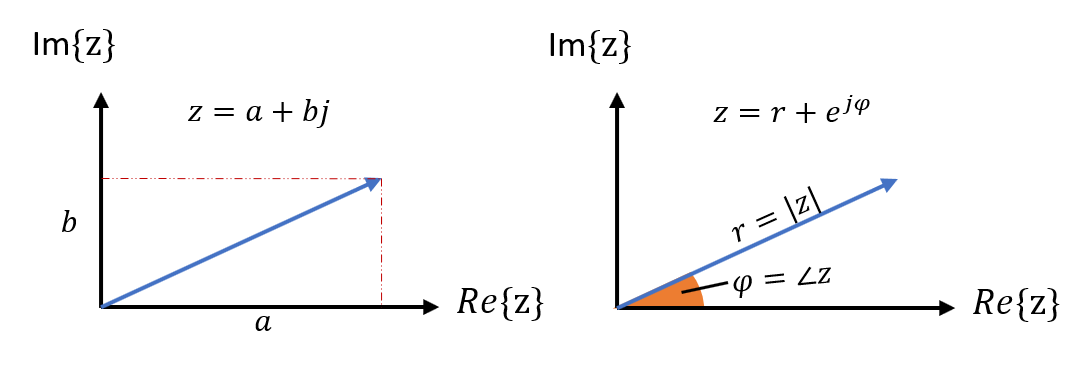
\includegraphics[scale=0.4]{img/komplex_numb.png}}
\end{center}
\iend

\definition{Argument einer komplexen Zahl}
\beginip
Das Argument einer komplexen Zahl bezeichnet den Winkel, welche zwischen dem Zeiger in der komplexen Ebene und der X-Achse eingeschlossen wird. \\
Bei einer komplexen Zahl $ \underline{Z} =  a + bj$ wird es folgendermassen berechnet: \\
\begin{center}

\begin{tabular}{cc}
 Bedingungen & Argument \\
\hline
\hline
$ a > 0 $ & $ Arg(\underline{Z}) = \angle \underline{Z} = tan^{-1}(\frac{b}{a})$ \\
\hline
$ a < 0 \ \& \ b \geq 0 $ & $ Arg(\underline{Z}) = \angle \underline{Z} = tan^{-1}(\frac{b}{a}) \mathbf{+} \pi$ \\
\hline
$ a < 0  \ \& \  b< 0 $ & $ Arg(\underline{Z}) = \angle \underline{Z} = tan^{-1}(\frac{b}{a}) \mathbf{-} \pi$ \\
\hline
\end{tabular}
\end{center}

\iend
\begin{center}

\end{center}


\newpage
\subsection{Zeiger}
\textbf{Zusammenhang komplexe Exponentialfunktion und Sinus}


Jeder Sinus kann als komplexe Exponentialfunktion geschrieben werden. \\
\formulaBegin
$ A \cdot sin(\omega t + \varphi) = Im\{\underline{Z} \cdot e^{j\omega t}\} $
\formulaEnd

\begin{center}
	\ibox{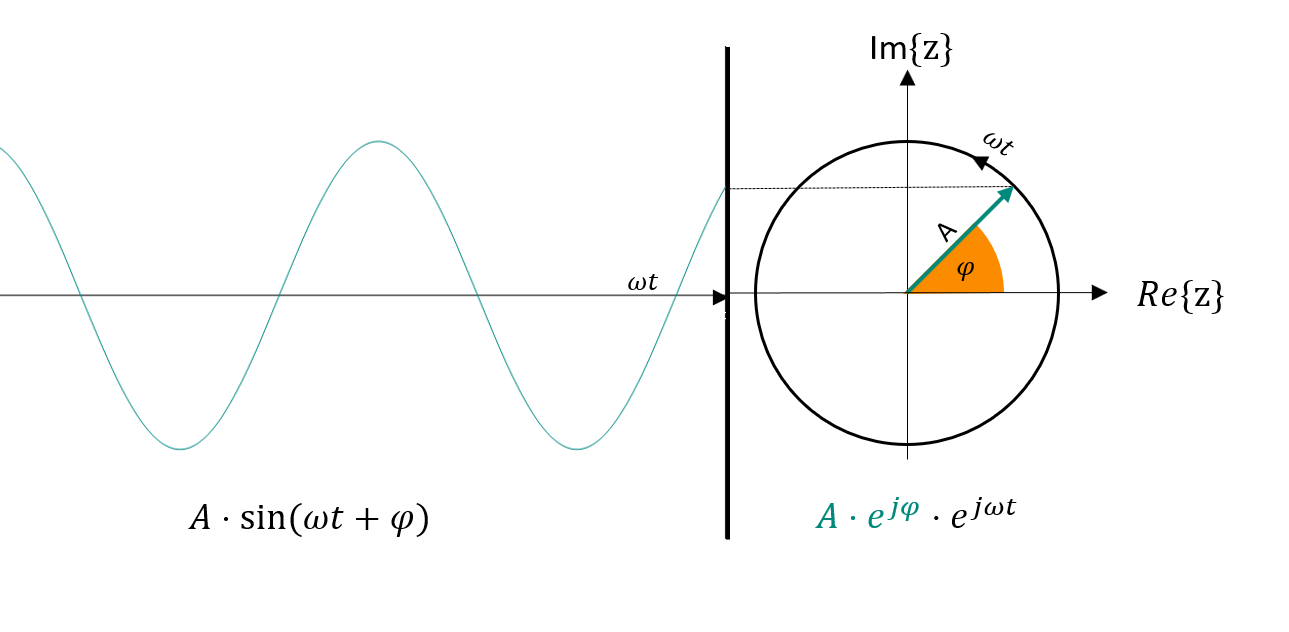
\includegraphics[scale=0.35]{img/sin-komex.png}}
\end{center}

Wir bezeichnen den \textbf{zeitunabhängigen Zeiger} mit Länge A und Winkel $\varphi$ als \textbf{komplexen Zeiger} (engl. Phasor). \\
Zusammen mit der Kreisfrequenz $\omega$ können wir den ihm zugrundeliegenden Sinus erhalten. \\

\definition{Zeiger}

\beginip
Ein \textbf{Zeiger} symbolisiert eine Sinusfunktion zum Zeitpunkt $t = 0$. \\
Folgende Eigenschaften gelten für einen komplexen Zeiger $\underline{\hat{u}}$
\begin{itemize}
\item $\underline{\hat{u}}$ ist zeitunabhängig
\item $\underline{\hat{u}}$ ist eine komplexe Grösse
\item $|\underline{\hat{u}}|$ entspricht dem Amplitudenwert des zugrunde liegenden Sinus
\item $ \angle \underline{\hat{u}}$ entspricht der Phasenverschiebung des Sinus
\end{itemize}

\iend

\newpage

\definition{Effektivwert und Gleichrichtwert}
\beginip
\textbf{Gleichrichtwert}  \\
Der Gleichrichtwert einer T-periodischen Funktion entspricht dem gemittelten Betrag über eine Periode \\
\formulaBegin
$\displaystyle \overline{|u|} = \frac{1}{T} \int_0^T |u| dt $
\formulaEnd



\textbf{Effektivwert}  \\
Der Effektivwert einer T-periodischen Funktion entspricht der 2-Norm gemittelt über einer Periode. \\
Er ist wichtig, da eine Gleichspannungsquelle mit dem Effektivwert der Wechselspannung gerade gleich viel Energie an einem Widerstand umsetzt, wie die Wechselspannung selbst. \\
\formulaBegin
$ \displaystyle  U = \sqrt{\frac{1}{T} \int_0^T u^2 dt} $
\formulaEnd
\iend

\vspace{1cm}
\textbf{Symbole und Bedeutung} \\
Nachfolgend sind ein paar Grössen aufgelistet, welche in Aufgaben und/oder Büchern verwendet werden. Sie beziehen sich stets auf ein sinusförmiges Eingangssignal. \\
 Eingangssignal: $ u(t) = A \cdot sin(\omega t + \varphi)$ \\
\begin{center}
\begin{tabular}{c|c}
 Symbol & Bedeutung \\
\hline
\hline
$\displaystyle \hat{u} $ &   Spitzen/Amplitudenwert des Sinus. $(= A)$ \\
\hline
$\displaystyle U$ & Effektivwert. Entspricht bei Sinusgrössen $\displaystyle  \frac{\hat{u}}{\sqrt{2}}$ \\
\hline
$\displaystyle \underline{U}$ & komplexer Zeiger (Effektivwert) mit Phase. $\displaystyle (= U \cdot e^{j\varphi t})$ \\
\hline
$\displaystyle \underline{\hat{u}}$ & komplexer Zeiger (Spitzenwert) mit Phase. $\displaystyle (= \hat{u} \cdot e^{j\varphi t})$ \\
\hline
\end{tabular}
\end{center}

\newpage

\definition{Komplexer Raum}

\beginip
Als Komplexen Raum bezeichne ich* den \textbf{zeitunabhängigen} Raum der komplexen Zeiger. \\
In diesem Raum werden zeitliche Ableitungen zu Multiplikationen und Integrale zu Brüchen. \\
Zwischen dem komplexen Raum und dem realem Raum sind folgende Zusammenhänge gegeben: \\

\begin{center}
\begin{tabular}{ccc}
 Realraum & komplexer Raum \\
\hline
\hline
$ \displaystyle u(t) = A \cdot sin(\omega t + \varphi) $ & $  \Rightarrow $ & $\displaystyle \underline{U}  = \frac{A}{\sqrt{2}} \cdot e^{j\varphi t} $ \\
\hline
$ \displaystyle u(t) = \sqrt{2} \cdot |\underline{U}| sin(\omega t + \angle \underline{U}) $ & $\Leftarrow$ & $ \underline{U} $\\
\hline
\end{tabular}
\end{center}
\begin{center}

\begin{tabular}{c|ll}
 Bauteil & Realraum & komplexer Raum \\
\hline
\hline
Widerstand R & $u(t) = R \cdot i(t)$ & $\underline{U} = R \underline{I}$ \\
\hline
Kapazität C & $ u(t) = \frac{1}{C} \int_0^t i(t) dt $ & $\underline{U} = \frac{1}{j\omega C} \cdot \underline{I} $ \\
\hline

Induktivität L & $ u(t) = L \frac{d}{dt} i(t) $ & $\underline{U} = j\omega L \cdot \underline{I} $ \\
\hline
\end{tabular}

\end{center}




\iend




\definition{Impedanz}
\beginip
Als Impedanz $\underline{Z}$ bezeichnen wir eine komplexe Zahl, welche Strom und Spannung im komplexen Raum über einem gewissen Bauteil in Verbindung setzt. \\
Umgangssprachlich wird sie auch als allgemeiner Widerstand bezeichnet. \\
\formulaBegin
$ \underline{U} = \underline{Z} \cdot \underline{I}$

\formulaEnd
\begin{center}

\begin{tabular}{c|l}


 Bauteil & Impedanz\\
\hline
\hline
Widerstand R & $\underline{Z} = R $\\
\hline
Kapazität C & $\underline{Z} = \frac{1}{j \omega C} $ \\
\hline

Induktivität L & $ \underline{Z} = j \omega L $ \\
\hline
\end{tabular}

\end{center}

\iend

\newpage



Mithilfe der Impedanz und den komplexen Zeigern können wir sämtlichen Grössen wie gewohnt berechnen, solange wir uns im komplexen Raum befinden. \\
Sämtliche gewohnten Konzepte wie Maschenregel, Knotenregel, Spannungs-/Stromteiler etc. können wie gewohnt angewandt werden. \\
Möchten wir also ein Netzwerk mit Wechselströmen berechnen, so transformieren wir zuerst das gesamte Netzwerk in den komplexen Raum, berechnen dort die gesuchten Grössen und transformieren danach das Ganze wieder zurück.\\


	\hspace{-0.8cm}
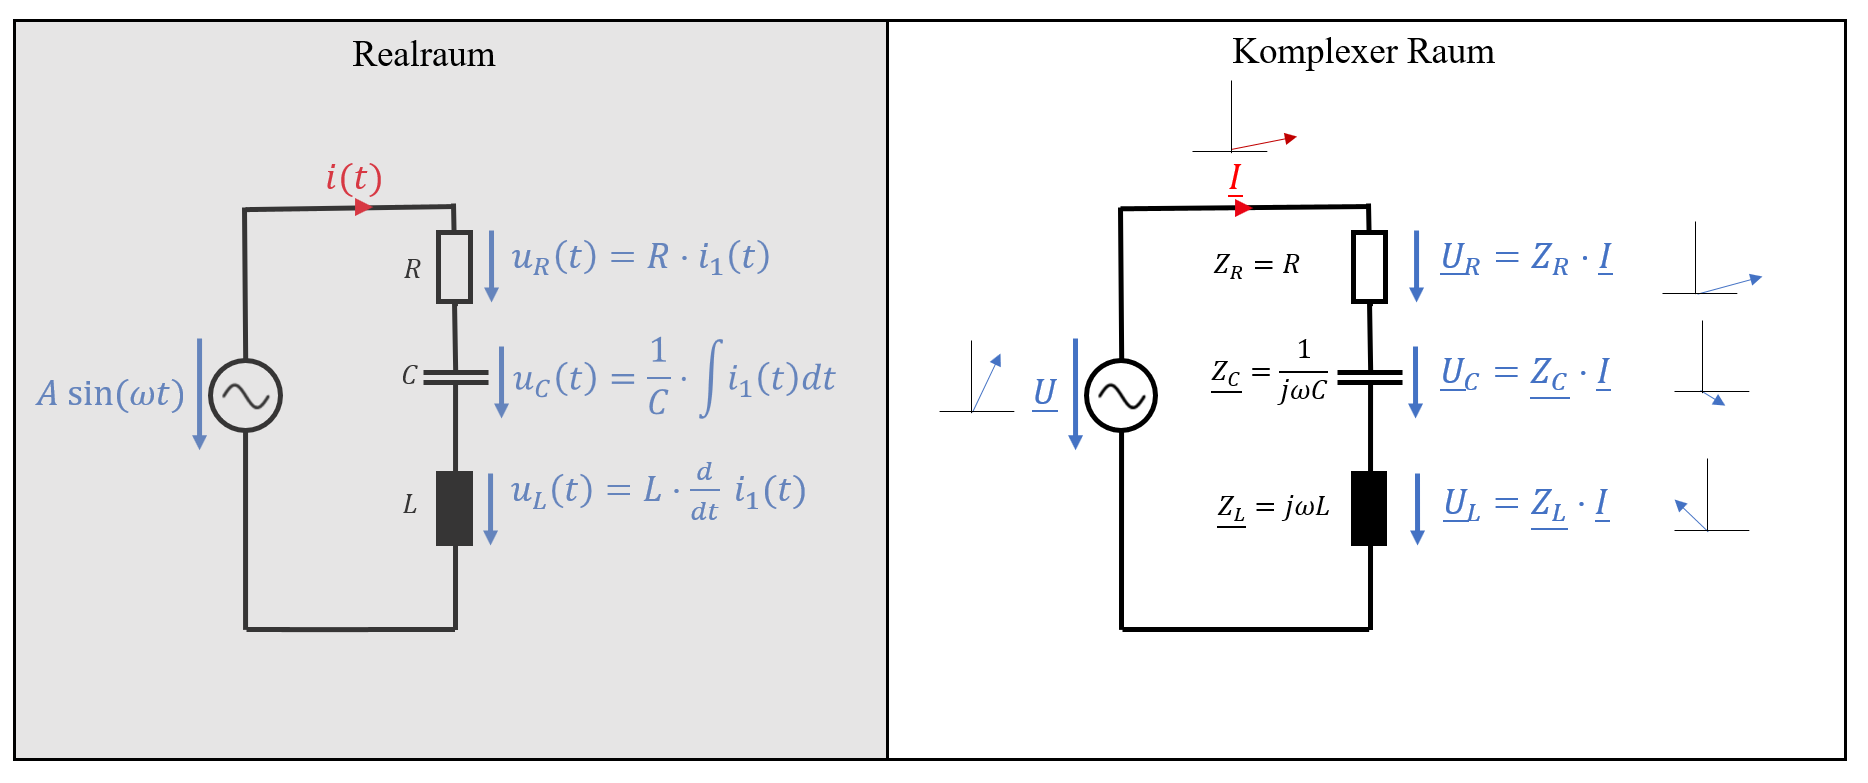
\includegraphics[scale=0.38]{img/komplexe_trafo.png}


\important{Beispiel}{\#6}
\beginip
Berechnen sie im folgenden Schaltbild der von der Quelle gelieferten Strom $i(t)$ und die Spannung über dem Kondensator $u_L(t)$ bei einer Eingangsspannung von $u(t) = 12V  sin(50\pi\cdot t)$
\begin{center}
	\ibox{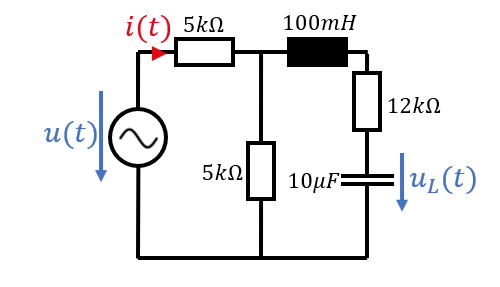
\includegraphics[scale=0.4]{img/ex6-1.png}}
\end{center}
\iend

\newpage

\important{Lösung}{}
\beginip
Zuerst transformieren wir sämtliche Grössen in den komplexen Raum: \\
$\displaystyle \underline{U} = \frac{12}{\sqrt{2}} $, $\displaystyle \omega = 50 \pi $ , $\displaystyle \underline{Z_C} = \frac{2000}{j \cdot \pi} \Omega $, $\displaystyle \underline{Z_L} = 5 \cdot \pi \cdot j \Omega $ \\
Nun berechnen wir den Gesamtwiderstand der Schaltung:\\
$\displaystyle \underline{Z_{ges}} = 5k\Omega + (5k\Omega || \underline{Z_L} + \underline{Z_C} + 12k\Omega) = 8531 - 53.64j = 8531.5 e^{-0.006\cdot j}  $ \\
$\displaystyle  \underline{I} = \frac{\underline{U}}{Z_{ges}} = \frac{12}{\sqrt{2} \cdot 8531.5} e^{0.006\cdot j} = 0.000995 \cdot e^{0.006\cdot j} A $ \\
$\displaystyle \Rightarrow \doubleunderline{i(t)} = \doubleunderline{6 \cdot sin(50\pi \cdot t + 0.34^\circ)} mA $  \\
Für die Spannung $\displaystyle u_L(t) $ : \\
Zuerst berechnen wir die Spannung über der Serienschaltung von Induktivität, Widerstand und Kondensator: \\
$\displaystyle \underline{U}_{serie} = \underline{U} \cdot \frac{(5k\Omega || \underline{Z_L} + \underline{Z_C} + 12k\Omega)}{\underline{Z_{ges}}} = (4.2423 - 0.0167 \cdot j) V = 4.242 \cdot e^{-0.00392 \cdot j}V $ \\
Daraus folgt für $\displaystyle \underline{U_c} $: \\
$\displaystyle \underline{U_C} = \underline{U}_{serie} \cdot \frac{\underline{Z_c}}{\underline{Z_L} + \underline{Z_C} + 12k\Omega} = (0.0108 - 0.2245)V = 0.225 \cdot e^{-0.1.523 \cdot j}V $ \\
$\displaystyle  \Rightarrow U_C(t) = 318 \cdot sin(50\pi \cdot t - 87.26^\circ) mV $
\iend


\newpage

\subsection{Zeigerdiagramm}
Als Zeigerdiagramm bezeichnen wir die Darstellung aller Spannungen/Ströme einer Schaltung in der komplexen Ebene. \\
Dabei müssen nicht alle Zeiger im Ursprung liegen, sie können auch beliebig verschoben werden. Einzig die Länge und der Phasenwinkel sind relevant. \\
Maschen- und Knotenregel müssen auch im Zeigerdiagram erfüllt sein. Dabei handelt es sich nun um Vektoradditionen der einzelnen Zeiger. \\

\textbf{Vorgehen} \\
Falls sämtliche Zeiger bereits berechnet wurden: \\
Alle Zeiger in Polarform umformen und vom Ursprung aus einzeichnen. \\
\\
Sonst: \\
\begin{enumerate}
	\item Wähle einen Massstab für Strom und Spannung. Achte darauf, dass auch der Zeiger mit der grössten Amplitude noch ins Bild passt. Falls alle Zeiger in nur einem Quadranten zu liegen kommen, kann möglicherweise der Rest des Plots weggelassen werden. Dies sieht man schnell anhand der Phasenverschiebung.
	\item Wähle einen Zeiger als Referenzzeiger. Zeichne ihn auf der reellen Achse ein.
	\item Alle anderen Zeiger werden nun der Reihe nach eingezeichnet, dabei müssen sie entsprechend ihrer Phasenverschiebung zum Referenzzeiger gedreht und entsprechend dem gewählten Massstab in der Länge skaliert werden. Es empfiehlt sich daher, die Phase aller Zeiger im Gradmass auszurechnen.
	\item Beim Zeichnen können und sollen bekannte Beziehungen wie die Maschen- und die Knotenregel unbedingt beachtet werden. Auch bekannte Winkel zwischen Strom und Spannung an den Bauteilen (-90,0 oder 90 Grad) können das Zeichnen deutlich vereinfachen.
	\item Zeiger können beliebig verschoben werden. Lediglich ihre Richtung und Länge ist entscheidend. Es macht also Sinn, die Zeiger möglichst intuitiv anzuordnen.
\end{enumerate}


\textbf{Beispiel einer Schaltung und Zeigerdiagramm} ($i_{R2}$ und $U_{R2}$ als Referenzzeiger)
\ibox{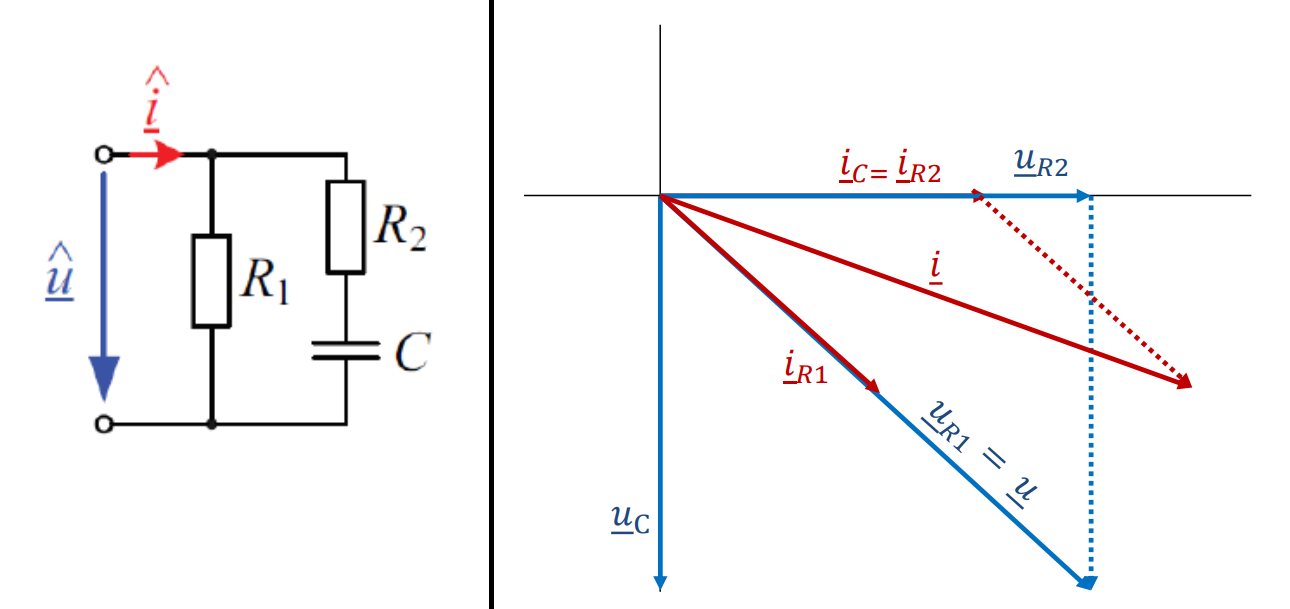
\includegraphics[scale=0.5]{img/zeigerdiag.png}}
\subsection{Komplexe Leistung}

\definition{Komplexe Leistung}
\beginip
Für eine beliebige Spannung $\underline{U}$ und  Strom $\underline{I}$ definieren wir die komplexe Leistung $\underline{S}$ als : \\
\formulaBegin
$ \underline{S} = \underline{U} \cdot \underline{I}^* = \underbrace{P}_{Wirkleistung} + \underbrace{jQ}_{Scheinleistung}$
\formulaEnd
\iend

\definition{Wirkleistung P}
\beginip
Als Wirkleistung bezeichnen wir Leistung, welche real von einem Verbraucher aufgenommen und in andere Leistungen (z. B. mechanische, thermische oder chemische) umgewandelt wird. \\
\formulaBegin
$P = Re\{\underline{S}\}$
\formulaEnd
\iend


\definition{Scheinleistung/Blindleistung Q}
\beginip
Als Schein-/Blindleistung bezeichnen wir Leistung, welche nur kurzfristig von einem Bauteil aufgenommen wird. Scheinleistung pendelt stets zwischen Quelle und Verbraucher hin und her und ist grundsätzlich unerwünscht. \\
\formulaBegin
$Q = Im\{\underline{S}\}$
\formulaEnd
\iend

\definition{Leistungsanpassung}
\beginip
Um maximale Leistung aus einem Netzwerk zu beziehen, muss der Lastwiderstand so gewählt werden, dass er gerade dem komplex konjugiertem der Innenimpedanz der Schaltung entspricht. \\
\begin{center}
	\fix \fix \fix
	\ibox{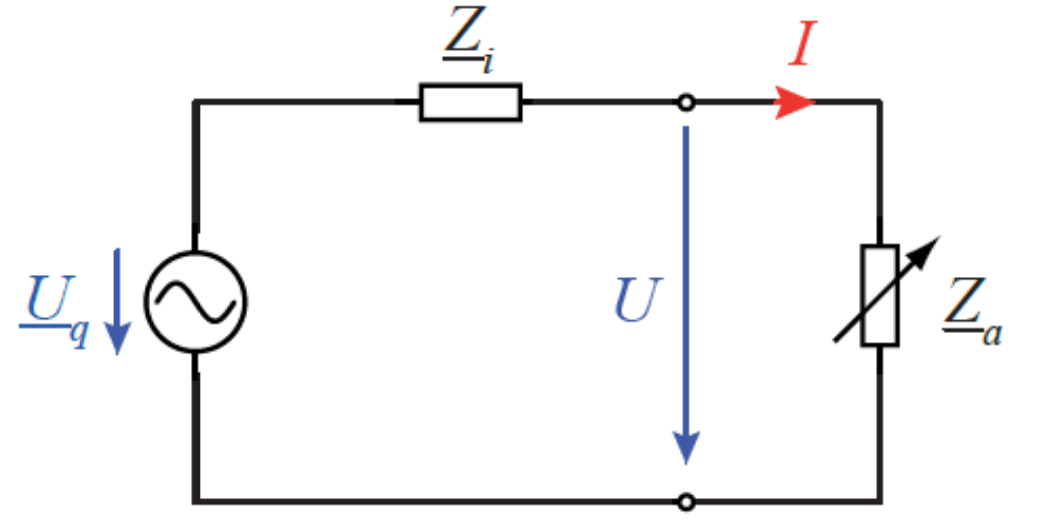
\includegraphics[scale=0.3]{img/koma_leistungsanp.png}}
\end{center}
\formulaBegin
$\underline{Z_a} = \underline{Z_i}^*$
\formulaEnd
\iend

\textbf{Begründung} \\
Wir möchten die Wirkleistung P maximieren und gleichzeitig die Blindleistung Q minimieren. \\
Für maximale Wirkleistung benötigen wir einen gleich grossen Lastwiderstand wie Innenwiderstand ($Re\{\underline{Z_a}\} = Re\{\underline{Z_i}\}$) \\
Um die Scheinleistung zu minimieren, müssen wir den Imaginärteil der Gesamtimpedanz minimieren, sodass $\underline{U}$ und $ \underline{I}$ in Phase sind. \\
$Im\{\underline{Z_a} +\underline{Z_i}\} = 0 \Rightarrow Im\{\underline{Z_a}\} = -Im\{\underline{Z_i}\}$


\newpage

\subsection{Schwingkreise}
Elektronische Bauelemente wie Kondensator und Spule speichern lediglich Energie, verbrauchen diese aber nicht. Hängen wir einen Kondensatoren und eine Spule zusammen, so pendelt die Energie vom einem Bauteil zum anderen.
Dieses Verhalten bezeichnen wir als Schwingkreis. \\

\begin{center}

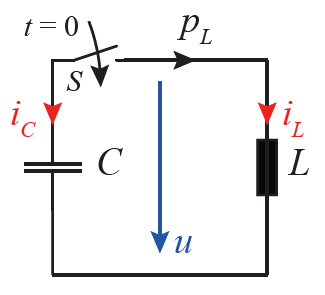
\includegraphics[scale=0.5]{img/schwingkreis.png}

\hspace{-3cm}
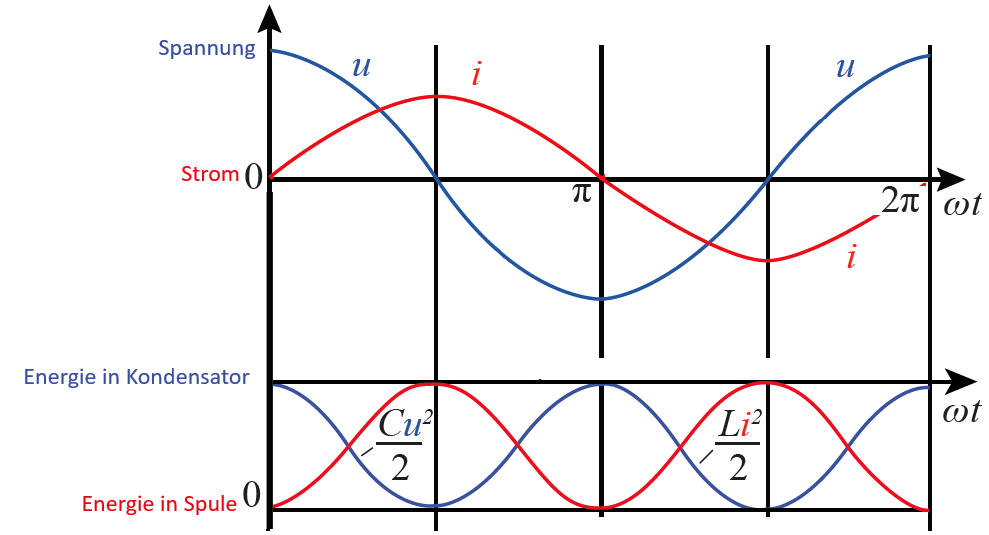
\includegraphics[scale=0.5]{img/schwingkreis_2.png}

\end{center}

Wir können nun die Schaltung mit einem Widerstand und einer Spannungsquelle erweitern: \\

\begin{center}
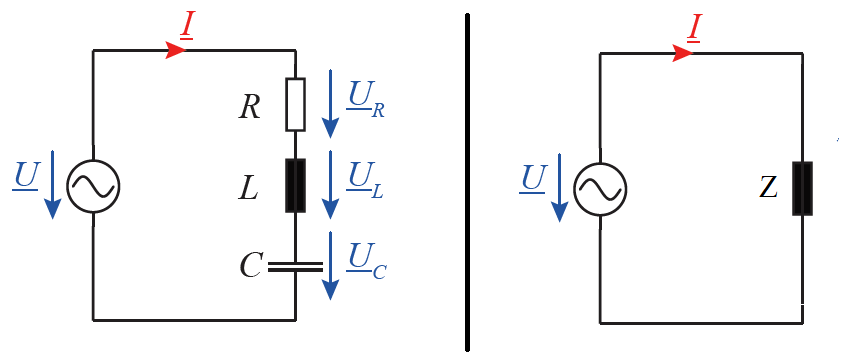
\includegraphics[scale=0.5]{img/schwingkreis_m_quelle.png}
\end{center}\

Ersetzen wir die Serienschaltung mit einer Impedanz, so erhalten wir für $\underline{Z}$: \\
\begin{center}

$\displaystyle \underline{Z} = R + j\omega L + \frac{1}{j \omega C} = R + j (\omega L - \frac{1}{\omega C})$ \\

\end{center}

Der Imaginärteil unserer Impedanz hängt also von der Frequenz unserer Quelle, der Kapazität und der Induktivität ab. \\
	Im allgemeinen Fall erhalten wir folgendes Zeigerdiagramm: \\
\begin{center}
\ibox{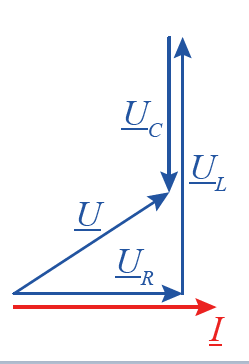
\includegraphics[scale=0.5]{img/zeiger_diag_1.png}}
\end{center}

Für den Fall, dass wir $\omega = \sqrt{\frac{1}{LC}}$ wählen, wird die Impedanz rein reell. Das Zeigerdiagramm sieht folgendermassen aus: \\
\begin{center}
	\ibox{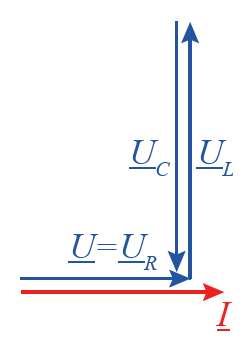
\includegraphics[scale=0.5]{img/zeiger_diag_2.png}}
\end{center}
Innerhalb dieser Schaltung treten massive hohe Spannungen ($U_L$, $U_C$) auf, welche von aussen \textbf{nicht messbar} sind und meist grösser als die Eingangsspannungen/Ströme sind.  \\
Dieses Verhalten bezeichnen wir als Resonanzverhalten.

\definition{Resonanzfrequenz}
\beginip
Betreiben wir eine Schaltung, welche sowohl eine Induktivität wie auch eine Kapazität beinhaltet, so existiert eine Eigenfrequenz bei welcher das System zu schwingen beginnt und die Spannungen oder Ströme über den Spulen/Kondensatoren rein imaginär wird. \\
Dies geschieht, sobald die Impedanz der Schaltung rein reell wird. \\
Die Frequenz $\omega_r$, bei welcher dieses Verhalten auftritt, lässt sich wie folgt berechnen:\\
\textbf{Alle Elemente sind Seriell / Parallel geschaltet}
\formulaBegin
$\displaystyle \omega_r := \sqrt{\frac{1}{LC}}$
\formulaEnd

\textbf{Bei einer Mischung aus seriell- / Parallelschaltungen}
\formulaBegin
$\displaystyle Im\{\underline{Z}(\omega_r)\}= 0 \Rightarrow \omega_r = ?$
\formulaEnd
\iend


\definition{Güte}
\beginip

Ein Mass dafür, wie gut ein Schwingkreis ist, ist die Güte Q. Sie ist definiert als das Verhältnis der im Schwingkreis gespeicherten Energie $W_{ges}$ und dem Energieverlust pro Periode $\Delta W$. \\
Der Gütefaktor sagt uns, wie stark ein System \textbf{gedämpft} ist bzw. wie schnell \textbf{Energie verloren geht}.\\
Zusätzlich sagt er etwas darüber aus, wie viel grösser die Spannungsüberhöhung im Verhältnis zur Eingangspsannung ist. \\
\formulaBegin
$\displaystyle Q = 2 \pi \cdot \frac{W_{ges}}{|\Delta W|} \underbrace{=}_{Q \gg 1} \frac{U_L}{U}$
\formulaEnd
\iend
